\documentclass[12pt,a4paper]{article}
\usepackage[utf8]{inputenc}
\usepackage[english]{babel}
\usepackage{setspace}
\usepackage{geometry}
\usepackage{graphicx}

\newgeometry{left=1in, top=1in, bottom=1in, right=1.5in}

\title{Space Debris Classification}
\author{Daniel Kolosa}
\date{04-20-2017}

\doublespacing

\begin{document}
\maketitle

\section{Introduction}
This project is a study to attempt to create a model to classify a portion of debris orbiting Earth. The first section is an itroduciton describing the backgound material, what is space debris and why is it an issue. The second section describes the dataset that is used for the statistical model and the model used. The third section will dicuss the statistical model itself and why it was chosen. The fourth section will look at the results obtained from the model and what conclusions can be drawn from the dataset and the model and the possible future work and implementations of this model.   

\section{Backgoround}
Ever since humans have been sending things into space we have not been cleaning up after ourselves. Sending things into space requires a lot of energy and cost, so bringing things back costs even more. The debris that is in space is the remains of dead satellites, rocket chasis, engines, components of space stations, and other micellaneous items. Fortunatly, some items that are close enough to Earth reenter the atmosphere are burn up on reentry, but there are still many objects that will remain in orbit for many years. The objects that will remain in orbit travel at very high speeds and can cause millions of dollars of damage if they collide with wokring space vehicles, or generate more debris if they collide with other objects.  

Before going into the statistical analysis methods used, the dataset used for this project will be discussed.
The dataset used is a collection of objects orbiting in the Low-Earth orbit (LEO) region. There are many other regions including, geo-synchronous orbit (GEO), high earth orbitl (HEO) but LEO orbit has a majority of the hazerdous debris. 

\section{Methods and Data}
%Satellite tracking data is encoded in a two line element set. The two line element set encodes position and velocity of a satellite based on its orbital elements. Orbital elements is a coordinate system used to describe the shape of an orbit. The two element set also includes data such as identification number, security classification either classified or unclassified epoch lauch dates, and atmospheric drag coefficients. The position and velocity of the objects are computed using simplified pertubation models. The simplified pertubation models are used to compute the orbital state of an object which taking into account the shape of the Earth, radiation, atmospheric drag, and gravitional influence from the Moon and Sun.

The dataset used for this project is provided by space-track.org. This organization collects and maintains datasets of satelliete position status and position data. The data is obtained from NORAD(North American Aerospace Defense Command) and NASA. The dataset will be analyzed using various methods. One interesting thing to look at is to see which countries have which objects. This is a good insight into what countries have what type of debris. The object type seen in this dataset are: debris, payload, rockect bodies, and others. Debris in this context consists of satellite and spacecraft fragments, payload is made up of capsulues of supplies or satellites. Rocket bodies consist of discarded roackets that were used to launch objects into orbit. 

Along with the object type the radar corss-section is an important metric to look at. The radar cross section is used to estimate the cross-sectional area of an object. For the purposes of this study, a larger radar cross section means that an object is larger. Speciic values for the radar cross section is not provided due to security reasons or lack of accuracy from the ground sttion sensors. Radar cross section is divided into three categories, small, medium, and large. Small are objects <$.1 m^2$, medium are objects between .1$m^2$ and 1$m^2$, and large objects are > $1m^2$.

The given dataset also provides orbital element data. The orbital element data provided are: apogee, perigee, inclination, and Period. The apogee and perigee are the maximum and minimum radii of an eliptical orbit, respectivly. The inclination is the tilt angle of the orbit relative to the Earth's equator and the period is the time it takes for the object to orbit the Earth in one revolution. 

Plots can help to narrow down which statistical models can be effective to analyze the dataset. The dataset provided contains not only debris but also other objects. The figure below shows what kind of objects and how many objects are in each category.
\begin{center}
	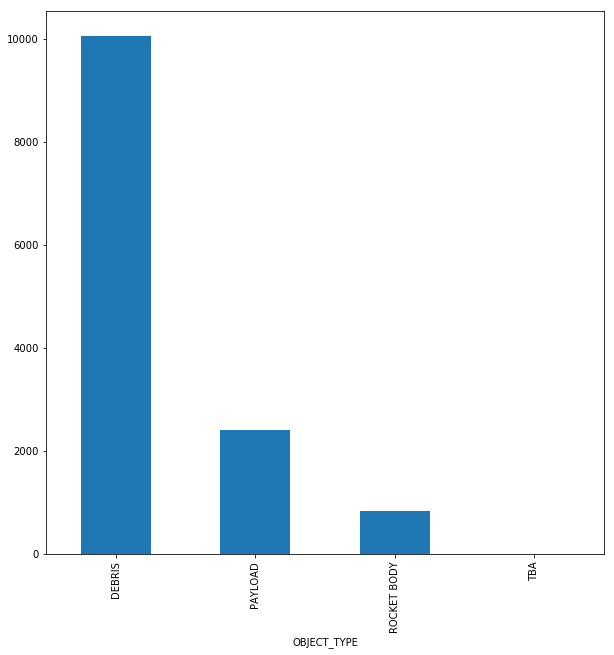
\includegraphics[scale=0.2]{figures/object_types.png}
	\captionof{figure}{Distribution of object size}
	\label{fig:object_types}
\end{center}
It can be seen from the figure above, that debris make up a significant amount of objects of the dataset. Another interesting plot to look at is the number of objects for the three different sizes.
\begin{center}
	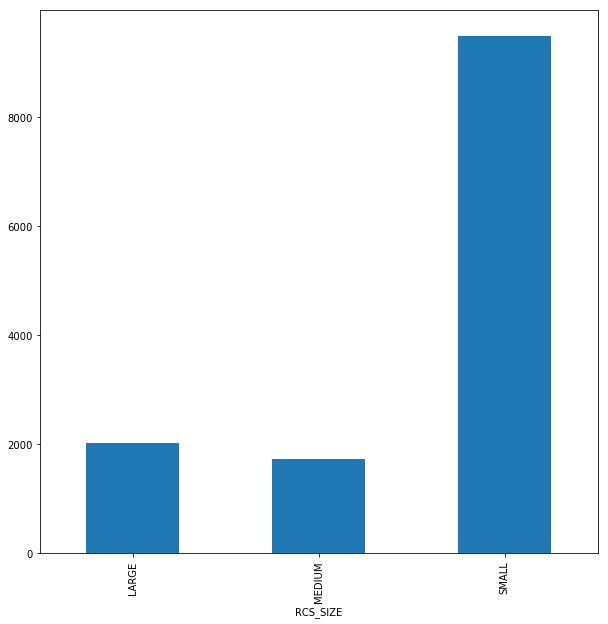
\includegraphics[scale=0.2]{figures/RCS_size.png}
	\captionof{figure}{Number of objects by object type}
	\label{fig:RCS_size}
\end{center}
Looing at the plot above, it can be seen that the most objects in the dataset have a small cross section. This gives a good visualization of what kind of debris are in orbit. 

Idealy, it would be best to have data that can tell us if an object is of high risk or low risk, but since there is no metric unsupervised learning will be used to investigate the data. Looking at the dataset provided, much of it is identification or launch data, so using PCA for feature extraction will not be necessary. Considering that the level of damage is a function of the amount of kinetic energy an object has, the mass and velocity are required. 
The dataset must go through some preprocessing before it can be used. The velocity can be approximated as the mean orbit sppedrom the equation below.
\begin{equation}
v = \frac{2a}{T}
\end{equation}
where T is the orbit period given by the dataset in seconds and a is the semimajor axis in kilometers, given in the equation below

\begin{equation}
a = \frac{r_p + r_a }{2}
\end{equation}
Where $r_p$ is perigee and $r_a$ is apogee.

Mass of objects are not given, but can be substituted with the size or radar cross section. Since radar cross section is classfied in small, medium, or large, this data must be converted into numeric data for a classifier to use. Useing one-hot encoding, a matrix is created to represent the sizes of the objects.
Since the dataset will be analyzed with unsupervised learning techniques, k-means clustering and a dendrogram will be used to analyze the selected features.    

\section{Results}

The number of clusters for the k-means classification is selected by measuring the disturbance at different values of clusters.
\begin{center}
	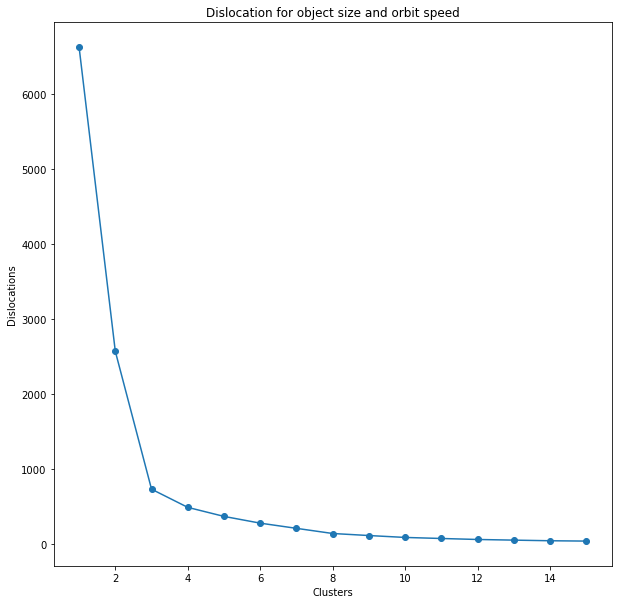
\includegraphics[scale=0.3]{figures/dislocation_obj_size.png}
	\captionof{figure}{Elbow Plot}
	\label{fig:Dislocation}
\end{center}
As seen in the figure above, using three or four clusters would be a good start for this situation. Using four clusters, a silhouette analysis is done. The silhouette plot will give an idea of the seperation distance between the clusters.
\begin{center}
	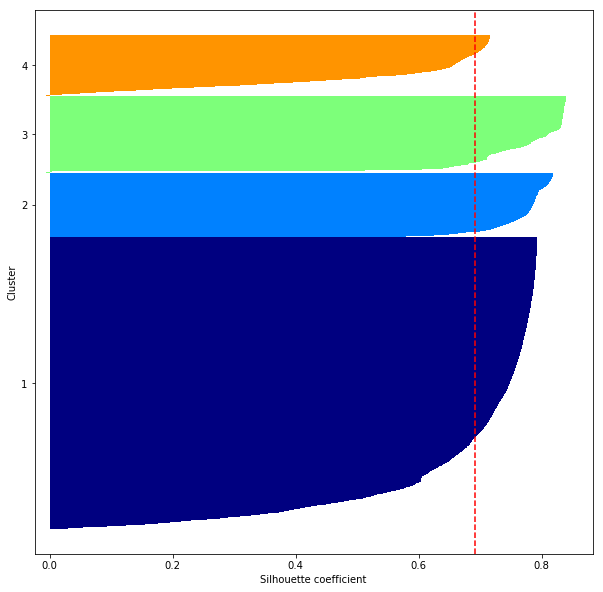
\includegraphics[scale=0.3]{figures/Silhouette.png}
	\captionof{figure}{Silhouette Analysis}
	\label{fig:Silhouette}
\end{center}
The Silhouette plot above shows a mean silhouette coefficient of 0.7 which is good degree of seperation, also with four clusters there is not much improvement in the silhouette coefficient, so in this case, using three clusters would be optimal.
The final method that will be looked at is a dendrogram plot. A dendrogram plot shows the correlation between the clusters in a dataset.
\begin{center}
	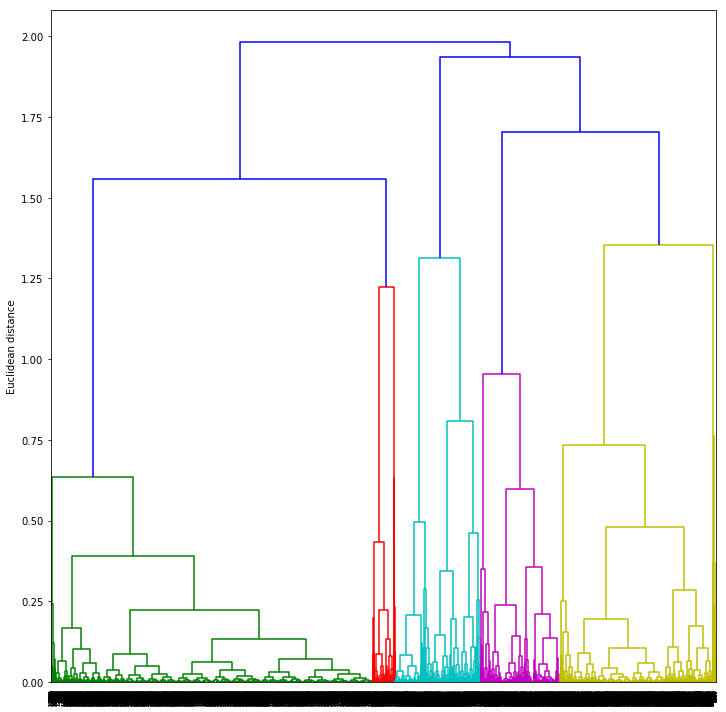
\includegraphics[scale=0.3]{figures/dendrogram.png}
	\captionof{figure}{dendrogram plot}
	\label{fig:dendrogram}
\end{center}
The dendrogram shows a high correlation between five different clusters. Looking at both the dendrogram and silhouette plots, there are no negative values meaning that there are no negative correlations. Also for are similar correlations for the clusters in green.
\section{Conclusion}
This papaer goes into the background inforamtion on space debris including the dangers and importance. Then the dataset was introducded and the prepocessing methods. Then the thinking behind selecting an unsupervised learning model was discussed. Finally a k-means classifier was analyzed using an elbow and a silhouette plot and a dendrogram to show the relasionship of the clusters.

The future work of this project could include implementing more complicated classification models like using neural networks. Also it would be beneficial to introduce drag models and get quantitative data on either size or mass to be a more accurate model 
 
 
\end{document}
